\chapter{Statistical Inference in fMRI}\label{chap:stats_fmri}
\markright{{~{\rm \ref{chap:stats_fmri}}. Statistical Inference in fMRI}\hfill}{}
\label{Chapter_2}



\vspace*{\fill}
\newthought{In chapter~\ref{chap:intro_fmri}}, we have presented fMRI as functional imaging modality that is non-invasive and enjoys good spatial resolution and full brain coverage. In this chapter we present the statistical methods that will be used for drawing conclusions from fMRI experiments in further chapters. 


The chapter is divided into two sections. The first section summarizes the basics of statistical hypothesis testing. We present two parametric test: the $t$-test and the $F$-test and one non-parametric test: the signed-rank Wilcoxon test. We discuss the voxel-wise parametric testing of the activation coefficients computed by the GLM. The result can be assembled into an image or map, a setting known as statistical parametric maps (SPMs).


The second section describes the basics of supervised machine learning. We introduce the supervised learning problem in the context of empirical risk minimization. We describe different surrogate loss functions and penalties that have found applications in the context of fMRI analysis. Finally, we present two applications of supervised learning to reveal cognitive mechanisms in fMRI studies. The first application is commonly known as \emph{decoding} or \emph{mind reading} and consist in predicting some information about the stimuli from the activation coefficients. The second application is known as \emph{encoding} and can be seen as the complementary operation of decoding: here, the activation coefficients are predicted from some information about the stimuli.


\hspace{20pt}
\begin{shaded}
Section~\ref{chap2_decoding} uses material from the following publication:
\begin{itemize}
\item V. Borghesani, F. Pedregosa, E. Eger, M. Buiatti, and M. Piazza, \emph{“A perceptual-to-conceptual gradient of word coding along the ventral path”} Proceedings of the 4th International Workshop on Pattern Recognition in Neuroimaging, 2014.
\end{itemize}
\end{shaded}
\vspace*{\fill}

\clearpage

\vspace*{\fill}
\minitoc
\vspace*{\fill}
\newpage

% This chapter relies on concepts from probability and measure theory that will be used without definition, such as \emph{probability space}, \emph{random variable}, \emph{population}, \emph{measurable function}, \emph{expectation}, etc. 

\section{Hypothesis testing}

A \emph{statistical hypothesis} is a statement about the parameter of a given distribution. The two complementary hypotheses in a hypothesis testing problem are called the \emph{null hypothesis} and the \emph{alternative hypothesis}. They will be denoted by $H_0$ and $H_1$, respectively. 


Given a random samples $\{x_1, \ldots, x_n\}$ drawn from a probability space $(\mathcal{X}, \mathcal{A}, P_{\theta})$, the goal of \emph{statistical hypothesis testing} is to decide, based on the random sample, whether it is possible to reject the presumed \emph{null hypothesis} $H_0$ for pre-specified level of significance. Let $\theta$ denote a distribution parameter, the general format of the null and alternative hypothesis is $H_0: \theta \in \Theta_0$ and $H_1: \theta \in \Theta_0^c$, where $\Theta_0$ is some subset of the parameter space and $\Theta_0^c$ is its complement. For example, if $\theta$ denotes the average activation of a voxel for a given condition, we might be interested in testing $H_0: \theta_0 = 0$ versus $H_1: \theta_0 \neq 0$ (or $H_1: \theta_0 > 0$).

% A \emph{hypothesis test} is a rule that specifies for which values of the sample space the decision is made to reject the null hypothesis or not. The subset of the sample space for which $H_0$ will be rejected is called the \emph{rejection region} or \emph{critical region}. Typically, given $(x_1, \ldots, x_n) \in \mathcal{X}^n$, a hypothesis test is specified in terms of a \emph{test statistic} $W(x_1, \ldots, x_n)$ = $W(\B{x})$. For example, a test might specify that $H_0$ is to be rejected if $\bar{\B{x}}$, the sample mean, is greater than 3. In this case, $W(\B{x}) = \bar{\B{x}}$ is the test statistic and the rejection region is $\{(x_1, \ldots, x_3) : \bar{\B{x}} > 3\}$.


\begin{marginfigure}
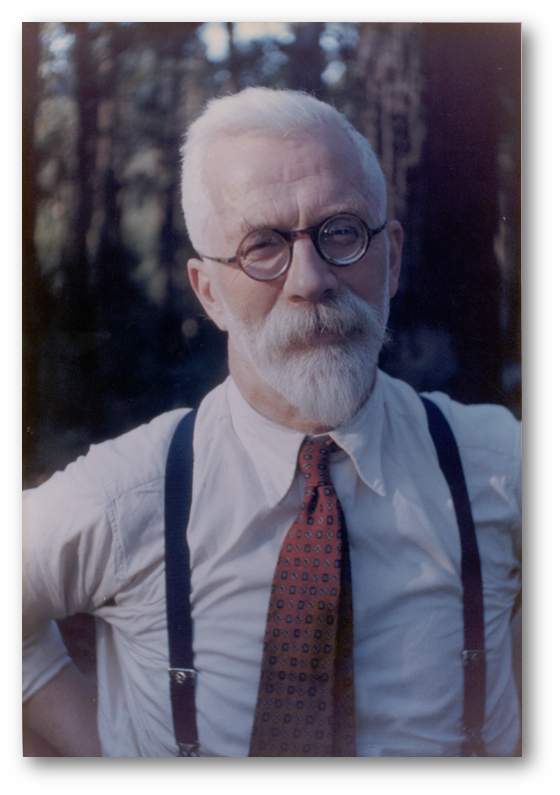
\includegraphics[width=1.\linewidth]{chapter_2/Fisher2.png}
\hspace{-20pt}\caption{Sir R. A. Fisher (London, England 1908 - Adelaide, Australia 1962) made important contributions to the field of statistics. Among many notions in statistic, he coined the terms ``test of significance'', ``Fisher consistency'' (which we will develop in Chapter 5) and ``null hypothesis''~\citep{fisher1925statistical}.}\label{fig:ronald_fisher}
\end{marginfigure}

The \emph{$p$-value} is a numerical quantity that serves to quantify the strength of the evidence against the null hypothesis and in favor of the alternative. Formally, the $p$-value is the probability of observing samples at least as favorable to the alternative hypothesis as the current samples, if the null hypothesis is true. Given a subset of the population, the $p$-value associated with a statistical test is usually computed by means of a function of these samples known as \emph{test statistic}.


Statistical tests can be broadly divided into \emph{parametric} and \emph{nonparametric} tests. Parametric test assume a known probability distribution for the distribution parameter that is under consideration. Nonparametric tests do not assume a known form of this probability distribution although they might require some regularity conditions on the distribution such as symmetry. In the following subsection we will describe two parametric statistical tests: the $t$-test and the $F$-test. In this thesis, the $t$ and $F$-test will be used to perform voxel-wise inference in section~\ref{subsec:spms}. We will also present the Wilcoxon signed-rank test, a nonparametric test that will be used to compare the performance of machine learning models in Chapter~\ref{chap:hrf_estimation} and Chapter~\ref{chap:decoding_ordinal}. The derivation of these tests is omitted but can be found in statistical textbooks such as~\citep{casella2002statistical, rice2006mathematical}.

\subsection{Parametric tests: $t$-test and $F$-test.}\label{subsec:parametric_tests}

\marginnote[-2cm]{Student was the pseudonym of Willian Sealy Gosset (England 1876 - England 1937). As a worker of the brewery Arthur Guiness \& Son he was forbidden to publish under his real name to protect the firm from its competitors. Gosset made important contributions to the field of small sample statistics. In the seminal paper \emph{The probable error of a mean}~\citep{student1908probable}, he introduced small sample estimation by means of the (Student) $t$-distribution family.}

The $t$-test is any statistical hypothesis test in which the test statistic follows a Student $t$ distribution under the null hypothesis. Most $t$-test statistics are of the form $t=Z/s$, where $Z$ and $s$ are functions of the samples, in which case the assumptions are: $Z$ follows a standard normal distribution, $s^2$ follows a $\chi^2$ distribution with $p$ degrees of freedom, and $Z, s$ are mutually independent. Once the $t$ statistic is determined, a $p$-value can be found from the values of a Student $t$ distribution with $p$ degrees of freedom.


The statistical test that has as null hypothesis that the population mean is equal to a specified value $\mu_0$ can be evaluated with a $t$-test known as the \emph{one-sample $t$-test}. Given a sample $\{x_1, \ldots, x_n\}$ of size $n$, the hypothesis
$$
H_0: \mu = \mu_0 \quad \text{versus} \quad H_1 : \mu \neq \mu_0 \quad.
$$
can be tested by performing a test that uses the test statistic
$$
t = \frac{\bar{\B{x}} - \mu_0}{ s / \sqrt{n}} \quad,
$$
where $\bar{\B{x}}$ is the sample mean, $s$ is the sample standard deviation of the sample and $n$ is the sample size. Once the test statistic $t$ has been computed, the test specifies to reject $H_0$ with significance level $\alpha$ if $t \geq t_d (1 - \alpha)$, where $t_d(1 - \alpha)$ is the $100 (1 - \alpha)$ percentile of the $t$ distribution with $d = n - 1$ degrees of freedom. 

A different test based on the $t$ distribution can be used to test the coefficients of a linear regression model. Given the equation
$$
\B{y} = \B{X}\bfbeta + b + \bfvarepsilon \quad,
$$
where $\B{X} \in \RR^{n \times p}$ is a given design matrix, $\bfbeta \in \RR^p$ and $b \in \RR$ are terms to be estimated and $\bfvarepsilon \in \RR^n$ is the error which follows a Gaussian $\mathcal{N}(0, \sigma^2 \B{I})$ distribution. It is desired to test that some linear combination of coefficients, $\B{c}^T \bfbeta$ with $\B{c} \in \RR^p$, is significantly different from zero, i.e., $H_0: \B{c}^T \bfbeta = 0 ~ H_1: \B{c}^T \bfbeta \neq 0$. In this case, the statistic
\begin{equation}
t = \frac{\mathbf{c}^T \hat{\bfbeta}}
{\hat{\sigma} \sqrt{\B{c}^T (\B{X}^T \B{X})^{-1} \B{c} }}
\label{Eq:c2_Ttest}
\end{equation}
follows a Student's distribution
with $n - (p + 1)$ degrees of freedom, where $(n, p)$ are the dimensions of the design matrix and $\hat{\sigma}^2$ is the estimate of the variance. 


The $F$-test can be seen as a generalization of the one-sample $t$-test to several groups. It can be used to asses whether the means of several pre-defined groups differ from each other. Given a total of $n$ observations, divided into $k$ groups of samples $\B{x}_1, \ldots, \B{x}_k$ with respective sizes $n_1, \ldots n_k$, a null hypothesis is of the form
$$
H_0 : \mu_1 = \mu_2 = \cdots = \mu_k \quad \text{versus} \quad H_1 : \text{at least one} ~\mu_i \neq \mu_j \quad,
$$
then the test statistic to test this hypothesis is calculated as the ratio between the between-group variability and the within-group variability:
\begin{equation}\label{eq:t_test}
F = \frac{\sum_i n_i (\bar{\B{x}}_i - \bar{\B{x}})^2 / (k-1)}{\sum_{ij} (\B{x}_{ij} - \bar{\B{x}}_i)^2 / (n - k)}.
\end{equation}

This statistic follows the $F$-distribution (also known as Snedecor's $F$ distribution or the Fisher–Snedecor distribution) with $(k-1, n-k)$ degrees of freedom under the null hypothesis, i.e. the null hypothesis can be rejected according to this test with significance level $\alpha$ if the F statistic is greater than $F_{(k-1, n-k)}(1 - \alpha)$, where $F_{(k-1, n-k)}$ denotes the $F$-distribution with $(k-1, n-k)$ degrees of freedom.

{As done previously for the $t$-test, a variant of the $F$-test can be used to test the coefficients of a linear regression model. In this case, instead of testing that a given contrast is significantly different from zero, we will test that a \emph{set of contrasts} are all simultaneously different from zero. In this case the contrast $\B{C}$ is a matrix with $k$ columns describing the possible linear combinations to be tested. For example, using a model with four parameters, to test whether all of them are equal to $0$, $H_0: \beta_1 = \beta_2 = \beta_3 = \beta_4 = 0$, one would specify a contrast of the form $\B{C} = \B{I}$, where $\B{I}$ is the identity matrix of size $4 \times 4$.

For an arbitrary contrast $\B{C}$, the $F$-statistic for this test is given by
$$
F = \frac{\text{Tr}(\B{C}\bfbeta \bfbeta^T \B{C}^T)}{
\hat{\sigma}^2 \text{Tr}({\B{C}^T (\B{X}^T\B{X})^{-1}\B{C}}) \quad,
}
$$
where the square root is taken element-wise. This expression follows an $F$ distribution with $r$ numerator and ${n - (p+1)}$ denominator degrees of freedom ($F_{r, n - (p+1)}$), where $r$ is the rank of $\B{C}$.
}

\subsection{Nonparametric tests: Wilcoxon signed-rank test.}\label{subsec:wilcoxon}


The \emph{Wilcoxon signed-rank} test can be used to asses whether two population means differ. That is, given the samples $\{x_1, \ldots, x_n\}$ and $\{y_1, \ldots, y_n\}$, we would like to test the following hypothesis $H_0: \bar{\B{x}} = \bar{\B{y}}, ~~ H_1: \bar{\B{x}} \neq \bar{\B{y}}$, where $\bar{\B{x}}$ is the sample mean, $\bar{\B{x}} = \frac{1}{n}\sum_{i=1}^n x_i$.


Because of this, it can be seen as a nonparametric alternative to the two-sample $t$-test. We will use the Wilcoxon signed-rank test to replace the two-sample $t$-test when the normality assumptions of the last are not met. The assumptions behind Wilcoxon signed-rank are that \emph{(a)} the two samples are paired (paired samples imply that each individual observation of one sample has a unique corresponding member in the other sample), and \emph{(b)} the distribution of the difference between the values within each pair must be symmetrical, i.e., the median difference must be identical to the mean difference. Beginning with a set of paired values $\B{x}_1$ and $\B{x}_2$, each of size $n$, the test statistic $W$ can be computed following the steps:
\begin{itemize}
\item calculate $|{x}_{1, i} - {x}_{2, i}|$ and $\text{sign}({x}_{1, i} - {x}_{2, i})$ for every $1 \geq i \geq n$. Exclude pairs which have zero difference.
\item order the remaining $n_r$ pairs from smallest absolute difference to largest absolute difference $|{x}_{1, i} - {x}_{2, i}|$.
\item rank the pairs, starting with the smallest as 1. Ties receive a rank equal to the average of the ranks they span. Let $r_i$ denote the rank.
\item calculate the test statistic $W = |\sum_{i=1}^{n_r} \text{sgn}({x}_{1, i} - {x}_{2, i}) r_i|$
\end{itemize}

As $n_r$ increases, the distribution of $W$ converges to a normal distribution. For small samples ($n_r < 10$), $W$ is compared to a critical value from a reference table.

%
% \subsection{Likelihood Ratio Tests}

% For a given hypothesis, different tests can be derived. The Neymann-Pearson lemma shows that the likelihood-ratio test is optimal.

% The \emph{likelihood ratio test} is a statistical test for making a decision between the null and alternative hypothesis based on the value of this ratio. Given a likelihood function $L(\theta|\beta)$ which is a function of the parameter $\theta$ with $\beta$ held fixed at the value that was actually observed, we defined the \emph{likelihood ratio} as
% $$
% \Lambda = \frac{ \sup\{ L( \theta | \bfbeta) : \theta \in \Theta_0 \}}{\sup\{ L(\theta | \bfbeta) : \theta \in \Theta \} }
% $$

% The likelihood ratio test rejects the null hypothesis $H_0$ when its inverse exceeds a critical value $\lambda_{\alpha}$. That is, the decision rule has the form:
% \begin{itemize}
% \item if $\Lambda^{-1} \geq \lambda_{\alpha}$~ reject $H_0$
% \item if $\Lambda^{-1} \geq \lambda_{\alpha}$~ do not reject $H_0$.
% \end{itemize}

% The rationale behind the 

% The critical value $\lambda_{\alpha}$ is usually chosen to obtain a specific significance level $\alpha$, through the relation $P_0(\Lambda \geq \lambda_{\alpha}) = \alpha$, where $P_0$ denotes the probability under the null hypothesis. The Neyman-Pearson lemma states that this likelihood ratio test is the most powerful among all level-$\alpha$ tests for this problem. The value of $\alpha$ is called the \emph{$p$-value} associated with the observation $\lambda_{\alpha}$ under the null hypothesis, and represents the chance under the null hypothesis of observing a test statistic $\lambda_{\alpha}$ as large or larger than actually observed.


% \begin{itemize}
% \item {\bf One-sample t-test}. In testing
% \end{itemize}



\subsection{Voxel-wise hypothesis testing: Statistical Parametric Maps} \label{subsec:spms}




Statistical Parametric Maps (SPMs)\sidenote{Statistical Parametric Mapping (SPM) can refer both to the set of techniques detailed in this section and to the SPM software distributed by the \emph{Wellcome Department of Imaging NeuroScience} at University College London.} are images with values that are, under the null hypothesis, distributed according to a known probability density function, usually Student $t$ or the $F$ distribution. To create such maps, one proceeds by performing a parametric test at each voxel. The resulting statistics are assembled into an image - the SPM. 

Given the activation coefficients for a single voxel $\beta \in \RR^k$ (cf. Section~\ref{chapter_1_GLM}), with $k$ being the number of conditions, it is possible to use a $t$-test to test whether  a given linear combination of the conditions is significantly different from zero. As we did in section~\ref{subsec:parametric_tests} we introduce the contrast $\mathbf{c}\in \RR^k$ so that $\mathbf{c}^T \bfbeta$ is a linear combination of the conditions. The hypothesis can then be written as $H_0: \B{c}^T \bfbeta = 0$, $H_1: \B{c}^T \bfbeta \neq 0$. In this case, under the assumptions of the $t$-test for the coefficients of a linear regression model (Gaussian and i.i.d noise in the \gls{GLM}), equation~\ref{eq:t_test} gives the expression of the statistic for this test. Assigning the statistic to every voxel creates an image with the same dimensions as the input brain images, in this case a the image is called a $t$-map because of the $t$-test used to generate it.


\begin{figure}
\begin{center}
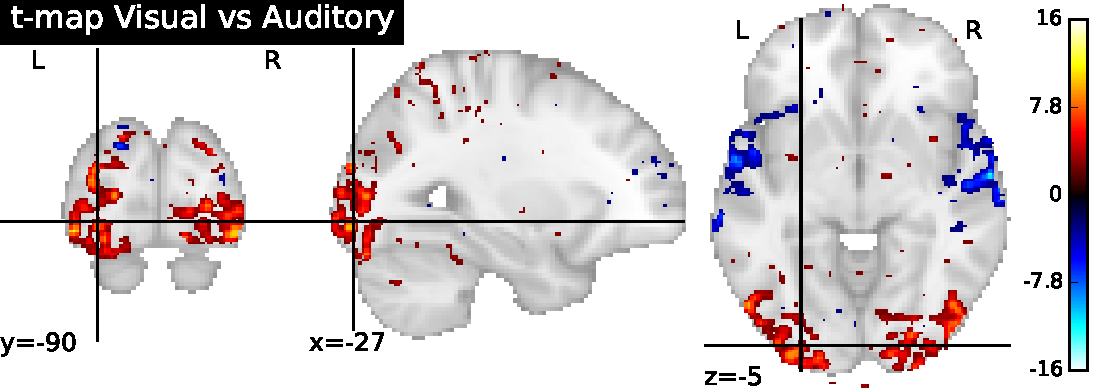
\includegraphics[width=.8\linewidth]{chapter_2/spm_visual_auditory.pdf}
\end{center}
% \vspace{-4ex}
\caption{$t$-map for a contrast of a Visual vs an Auditory task. Thresholded at $p$-value $< 10 ^ {-3}$. It can be seen how the voxels that exhibit a higher significance of this contrast belong to visual areas (red) and auditory areas (blue).}\label{fig:t_test_localizer}
\end{figure}


Figure~\ref{fig:t_test_localizer} plots the $t$-map resulted from a functional localizer~\citep{pinel2007fast} performed as part of the acquisition in~\citet{borghesani:hal-00986606} dataset. For this, the conditions `Visual' and `Auditory' were compared. Since only two conditions were compared, the contrast is of the form $\B{c} = [+1, -1, 0, \ldots, 0]$ where the entry $+1$ is for the Visual condition and $-1$ for the auditory condition. The image is thresholded so that only voxels with a $p$-value smaller than $10^ {-3}$ are displayed. It can be seen how the voxels that exhibit a higher significance of this contrast belong to visual areas (red) and auditory areas (blue) [see Figure~\ref{fig:chapter_1_functions} for a localization of some brain regions]. This example involves the testing of a single contrasts using a $t$-statistic. In similar fashion, the test in which we consider $d$ contrasts, i.e. $H_0: \B{c}_1^T \bfbeta$ = $\B{c}_2^T \bfbeta$ = $\cdots$ = $\B{c}_d^T \bfbeta$ = 0 and $H_1:$ at least one $\B{c}_i^T\bfbeta \neq 0$ can be performed using an $F$-test as described in section~\ref{subsec:parametric_tests}.



% \subsection{Permutations testing}

% {\blue 
% Discuss parametric and nonparametric. \citep{nichols2002nonparametric, goodpermutation} and Polina for the classification side. 
% % Stuff in here http://www2.warwick.ac.uk/fac/sci/statistics/staff/academic-research/nichols/software/snpm/#Refs
% }


% In order to perform hypothesis testing, we need to know the probability distribution of the selected statistic under the null hypothesis. For example, the previously mentioned $t$-test assumes the probability density of the statistic is the Student distribution. However, deriving a parametric distribution for a particular statistic requires making strong assumptions on the generative model of the data. Consequently, nonparametric techniques, such as \emph{permutation tests}~\citep{goodpermutation}, can be of great value if the distribution of the data is unknown.


% Permutation testing can be traced back to at least Fisher (XXX 1935, Chapter 3). Instead of comparing the actual value of a test statistic to a standard statistical distribution, the reference distribution is generated from the data themselves, as described below. 

% {\blue Good reference~\citep{golland2003permutation}}

% the theoretical distribution of the test statistic may only be known under particular assumptions that may be be violated in practice. The specificity of the test is then impacted. Alternatively, one may want to use a specificc test statistic, the theoretical distribution of which is not known under the null hypothesis. This is likely to happen for computational reasons for instance. The Monte-Carlo method [33] can be used to empirically approximate the unknown distribution: N artificial datasets are created on the model of the original data under the null hypothesis, so that N realizations of the test statistic are observed. However, it is difficult to reproduce the real-data problem with simulations. Permutation testing can be seen as a way to build the unknown H0 distribution from the observed data. Those are transformed in such a way the decision statistics' distribution remains the same under the null hypothesis, 


\subsection{Multiple comparisons issues}




One major drawback of statistical parametric maps is the multiple comparisons issue. This occurs when multiple hypothesis tests are performed simultaneously and one must account for the possibility of errors occurring on each of these tests~\citep{toothaker1993multiple, miller1966simultaneous, westfall1993resampling}. In fMRI, due to the huge amount of voxels (on the order of $4 \times 10^4$ at $3mm^3$ resolution), some tests can lead to a large amount of false positive results, i.e., some voxels are found to be significant while in reality they were not. As a result, it is necessary to consider other types of error rates which account for the multiple comparisons issue. 

A simple procedure to control the rate of false positives is through the \emph{Bonferroni correction} method. This approach consists in dividing the threshold $\alpha$ by the number
of tests $p$, which yields the new threshold $\alpha_b = \alpha / p$.
%  Indeed, in order to have a global test (brain-wide test) with a significance
% level of $\alpha$ (\emph{i.e.} a probability of incorrectly rejecting the null
% hypothesis of $\alpha$), the different tests (voxel-wide tests) have to be
% performed with a very low significance level $\alpha/p$, where $p$ is the
% number
% of unitary tests.
The maps of voxels selected by thresholding the \emph{$p$-values} for the object
recognition task (subject 1), are given in Fig.\ref{fig:chapter_2_comparisons},
for different threshold values ($0.05$, $0.01$ and $0.05$ corrected by
\emph{Bonferroni}).
We notice that \emph{Bonferroni correction} is very severe, and that
it keeps very few significant voxels. 

\begin{figure}
\begin{center}
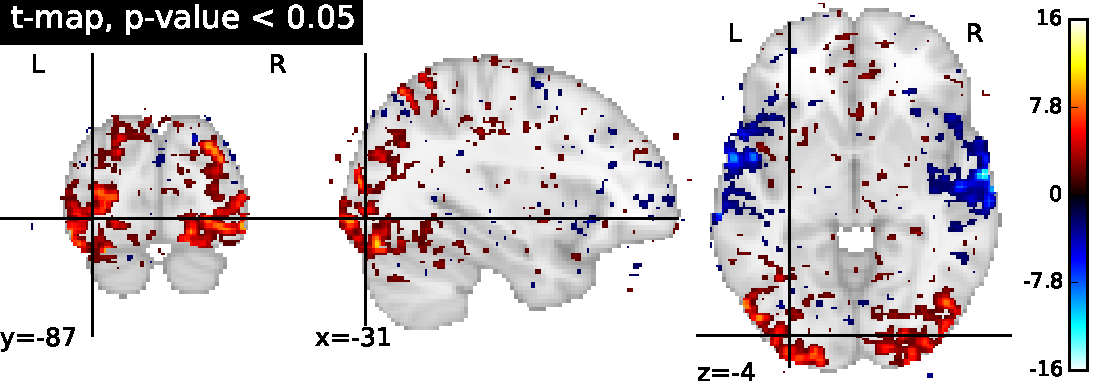
\includegraphics[width=.8\linewidth]{chapter_2/spm_visual_auditory_pval005.pdf}
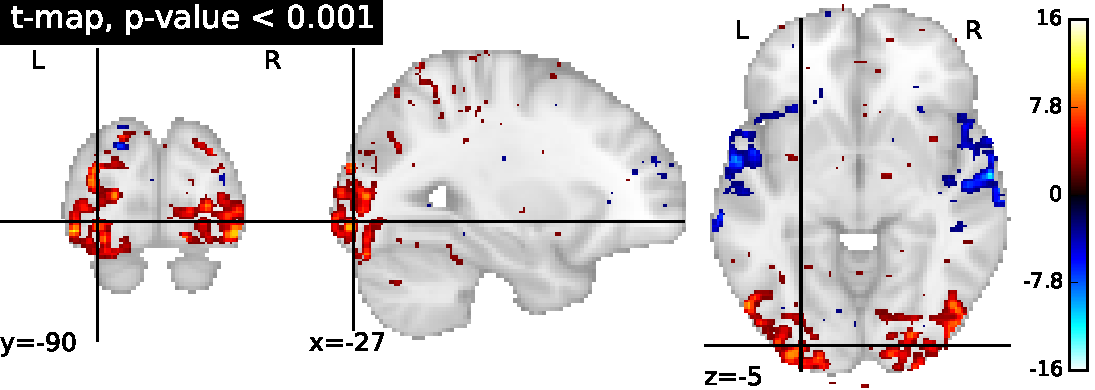
\includegraphics[width=.8\linewidth]{chapter_2/spm_visual_auditory_pval001.pdf}
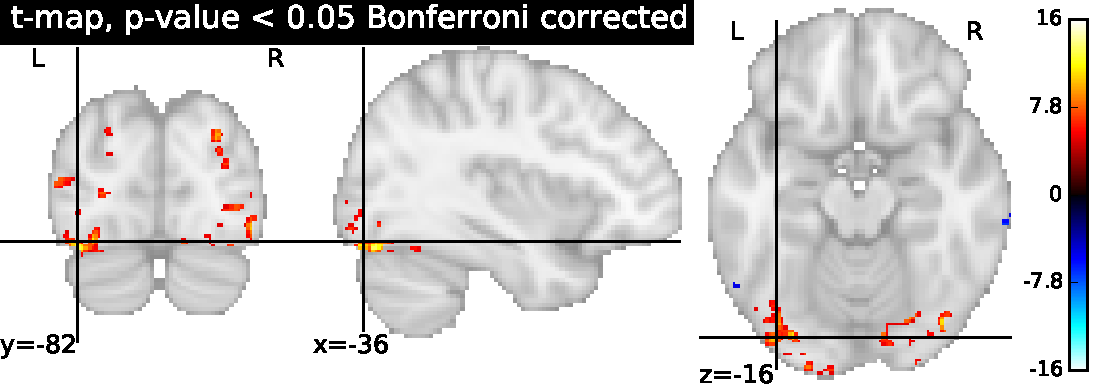
\includegraphics[width=.8\linewidth]{chapter_2/spm_visual_auditory_pval005_corrected.pdf}
\end{center}
% \vspace{-4ex}
\caption{\emph{Visual vs Auditory contrast}. Visualization of the voxels selected by
thresholding the
\emph{$p$-values} for the Visual vs Auditory contrast at different thresholds
($0.05$, $0.01$ and $0.05$ corrected by \emph{Bonferroni}). The \emph{Bonferroni
correction} is very severe and keeps very few voxels.
}\label{fig:chapter_2_comparisons}
\end{figure}


One of the main limitations behind Bonferroni corrections is that it does not take into account the spatial structure of the SPM. As such the number of independent test can smaller than the number of voxels. 
% Because of this, Bonferroni correction is widely regarded as being too conservative.
Other approaches besides Bonferroni correction include random field theory~\citep{friston1994assessing, worsley1992three} and resampling techniques~\citep{Friman2005859, holmes2003bootstrapping}. The review papers~\citep{Logan200495, Nichols2012811} provide an overview of the different methods that have been proposed to overcome this problem.



\section{Machine learning in fMRI}

\newglossaryentry{decoding}{name=decoding,description=distinguish patterns of neural activity associated with different stimuli or cognitive states}
\newglossaryentry{encoding}{name=encoding,description=predicting patterns of brain response to novel stimuli based on their features}


While classical statistical modeling emphasizes statistical inference (confidence intervals, hypothesis test, optimal estimators), the field of \emph{machine learning}, also known as statistical learning and pattern recognition, emphasizes model validation as measured by its performance on unseen samples. That is, in machine learning the validity of an estimated model will be judged based on its generalization performance. 

The first applications of machine learning to neuroimaging focused on distinguishing patterns of neural activity associated with different stimuli or cognitive states, a problem commonly known as \emph{\gls{decoding}}, \emph{reverse inference} or \emph{brain reading}~\citep{dehaene1998inferring, cox2003,laconte2005support, thirion2006, Sutao2011} uses a machine learning model to discriminate patterns of neural activity associated with different stimuli or cognitive states. In this thesis we will also  describe the~\emph{encoding} problem~\citep{thirion2006, Kay2008, mitchell2008predicting}, in which the patterns of brain activity are predicted based on the stimuli features. Encoding and decoding can be seen as complementary operations: encoding uses stimuli to predict activity while decoding uses activity to predict information about the stimuli. We will further describe these settings in Section~\ref{chap2_decoding} and \ref{chap2_encoding}, respectively.


% {\blue In this thesis we focus on supervised learning models, i.e. models in which the training set contains samples and labels. Other machine learning settings include unsupervised learning (where the training labels are not available), semisupervised learning (where only a fraction of the training labels are available) and reinforcement learning (where a fraction of the training samples and its respective target values are obtained during the learning process). The models that we will use in this thesis will belong to the supervised learning setting }.



% The shift from univariate methods to multivariate methods also entails a change in the questions that can be asked to fMRI studies. While univariate methods ask the question of which regions of the brain which are more active for one condition compared to another, multivariate methods can ask what information is represented in a region in terms of brain states associated with distinct patterns of activity, and how that information is encoded and organized~\citep{Haxby2012}.

\subsection{Supervised Learning}\label{subsec:supervised_learning}

Supervised learning is the task of learning a function from labeled training data. We will now give a formal definition of the task. 

We consider two spaces $\mathcal{X}$ and $\mathcal{Y}$. We will refer to $\mathcal{X}$ as the \emph{sample space} and to $\mathcal{Y}$ as the \emph{target space}. We assume that the pair $(X, Y)$ is a random variable taking values in $\mathcal{X} \times \mathcal{Y}$ and distributed according to an \emph{unknown} probability distribution $P$.  We observe a sequence of $n$ i.i.d. pairs  $\{(x_1, y_1), \ldots, (x_n, y_n)\} \in (\mathcal{X} \times \mathcal{Y})^n$ sampled according to $P$ and the goal is to construct  a function $h: \mathcal{X} \to \mathcal{Y}$ which \emph{predicts} $Y$ from $X$.

We need a criterion to choose this function $h$. For this we are given a \emph{loss function} $\ell: \mathcal{Y} \times \mathcal{Y} \to \RR$ that measures the disagreement between a pair of elements in the target space. This way $\ell(y_i, f(x_i))$ quantifies the penalty of predicting the target $f(x_i)$ when the true label is $y_i$. The objective is to construct a function $h$ such that its \emph{risk} is as small as possible. The risk of a function $h$ is defined as:
$$
\mathcal{R}(h) = \mathbb{E}_{X \times Y}(\ell(Y, h(X)))
$$

A function that achieves the minimum risk over all possible measurable functions is called the \emph{Bayes predictor} and is denoted $h^*$:
$$
h^* \in \argmin_h \mathcal{R}(h)
$$



However, in general the risk cannot be computed because the distribution $P$ is unknown. As an alternative we can use an approximation of the risk, called the~\emph{empirical risk}, by averaging the loss function over the pairs $\{(x_1, y_1), \ldots, (x_m, y_m)\} \in (\mathcal{X} \times \mathcal{Y})^m$ drawn from $P$. The empirical risk is defined as: 
\begin{equation}\label{eq:empirical_risk}
{{\mathcal{R}}_n}(f) = \frac{1}{n} \sum_{i=1}^n \ell(y_i, f(x_i)) \quad.
\end{equation}

% {\blue In this case the $n$ elements $\{X_1, X_2, \ldots, X_n\}$ in the training set can be represented as a $n \times p$ matrix, $\B{X} \in \RR^{n \times p}$ and the $n$ target elements from the training set $\{y_1, y_2, \ldots, y_n\}$ can be represented as a vector $\B{y} \in \RR^n$.}

\begin{marginfigure}
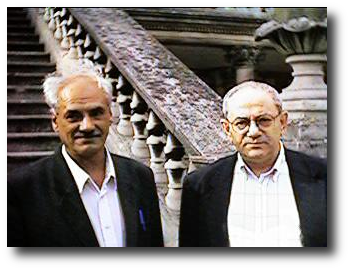
\includegraphics[width=\linewidth]{chapter_2/vc.png}
\caption{Vapnik–Chervonenkis theory (also known as VC theory) was developed during 1960–1990 by Vladimir Vapnik (right) and Alexey Chervonenkis (left). The theory attempts to explain the learning process from a statistical point of view.}
\end{marginfigure}

The task is then to find the function $f$ that minimizes the empirical risk, a setting known as \emph{empirical risk minimization}~\citep{vapnik1974teoriya}. Although the methods studied in this thesis can be seen within the framework of empirical risk minimization, several alternatives exist to this framework. A different setting for the estimation of learning models is \emph{maximum likelihood estimation}, in which the model parameters are chosen as the maximizers of the likelihood function. When the loss function $\ell$ can be written as the negative log likelihood: $\ell(y, f(x)) = -\log P(f(x)|x)$, then empirical risk minimization is equivalent to maximum likelihood estimation.

\paragraph{Classification.} If the target space $\mathcal{Y}$ is a finite set then the learning problem is known as \emph{classification}. In the special case that this target space contains only two different values, then this problem is known as \emph{binary classification}. The common loss $\ell$ in this setting is the zer-one loss, defined as $\ell(y, \hat{y}) = 0$ if $y = \hat{y}$ and $0$ otherwise.

\paragraph{Regression.} If on the other hand the target space is identified with an interval of $\RR$ we speak about a \emph{regression} problem. For example, the task of predicting the gender of a person would be a (binary) classification task since only two outcomes are possible. On the other hand, the task of predicting the height of a person is considered a regression task since the target space is an interval from the real line. The encoding and decoding problems in fMRI that we will consider in this chapter can be framed either using classification or regression models. The \emph{pairwise ranking} and \emph{ordinal regression} models that we will consider in Chapter~\ref{chap:decoding_ordinal} and \ref{chap:consistency} can be seen as a special case of classification problems in which the loss function depends on the distance between the respective labels. As we will see in Chapter~\ref{chap:decoding_ordinal}, one of the contributions of this thesis is to show that certain decoding problems can be formulated using ranking and ordinal regression models rather than multiclass or regression. 

For most practical applications, the sample space $\mathcal{X}$ is identified with $\RR^p$, where $p$ is referred to as the \emph{dimensionality} or \emph{number of features} of the learning problem and the target space $\mathcal{Y}$ is identified with $\RR$.




\subsection{Surrogate loss functions.}\label{subsec:surrogate_loss_functions}

\begin{marginfigure}[2cm]
\hspace{-20pt}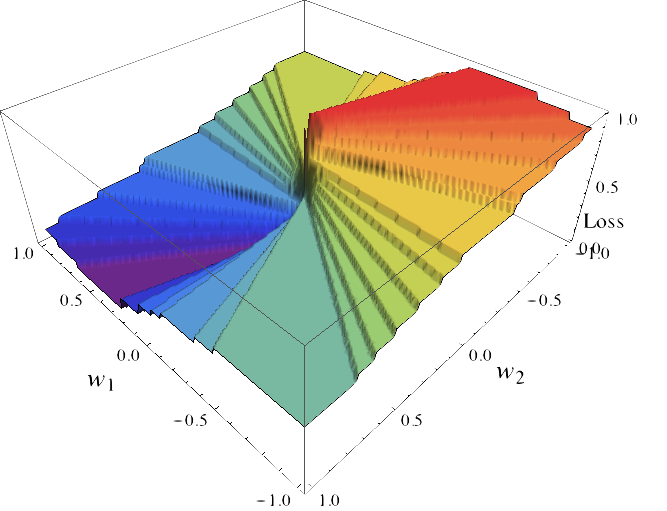
\includegraphics[width=1.2\linewidth]{chapter_2/loss_01.png}
\vspace{-10pt}\caption{
	The direct minimization of the empirical risk for the 0-1 loss is a difficult computational problem due to the discontinuity of and non-convexity of the loss function. In the figure: plot of the surface $g(w_1, w_2) = \mathcal{R}(f)$, where $f$ is the linear classification function $f(\B{x}) = \sign(\B{x}^T \B{w})$ with $\B{X} \in \RR^{10 \times 2}$ a random normally distributed matrix.
	This surface is discontinuous with large, flat regions and is thus not amenable for optimization using gradient-based methods.
}\label{fig:01_minimization}
\end{marginfigure}

\newglossaryentry{Heaviside}{name=Heaviside,description=The real function that is zero for negative values and one otherwise}


The direct minimization of the empirical risk is often not a tractable optimization problem. For example, consider the binary classification 0-1 loss, defined as
$$
\ell_{0-1}(y, \hat{y}) = \mathcal{H}( - y \cdot \hat{y}) \quad,
$$
where $\mathcal{H}$ is the \gls{Heaviside} step function, defined as $\mathcal{H}(x) = 1$ if $x \geq 0$ and $0$ otherwise.
Minimization of the empirical risk associated with this loss is known to be NP-hard even for the class of functions as linear classifiers. See Figure~\ref{fig:01_minimization} for an informal justification and \citep{feldman2012agnostic} and reference therein for a formal discussion of these properties. 

For this reason it is common to consider instead a function ${\psi: \mathcal{Y} \times \RR^d \to \RR}$ which is an approximation to the true loss known as \emph{surrogate loss} function. $d$ is an integer that will be determined by the surrogate loss function. For binary classification, $d$ is usually 1, while for multiclass classification $d$ is usually equal to the number of classes. The goal in this setting is to minimize the empirical $\psi$-risk, defined as
$$
{\mathcal{R}}_{n}^{\psi}(g) = \frac{1}{n} \sum_{i=1}^n \psi(y_i, g(x_i)) \quad.
$$
For computational reasons, $\psi$ is often a convex function in its second variable (the variable with respect to which we will minimize). Note that in this case the function $g$ has as output space $\RR$ and not $\mathcal{Y}$ as was the case before, thus the function $g$ is not a prediction function. In binary-class classification, the prediction of two classes is given by the sign of this function. In this case, we will call $g$ a decision function and $\text{sign}(g(X))$ will be the prediction function while in multiclass classification the prediction function is usually given by $\argmax_{c \in \{1, \ldots, k\}} g_i(x)$ \citep{Zhang2004}.


Compared to the empirical risk minimization setting, we have replaced the original problem by one with better computational properties. It is natural to ask whether what have we lost in the process. In Chapter~\ref{chap:consistency} we will present results on the consistency of surrogate loss functions, that is, under which conditions minimizing the $\psi$-risk leads to the same solution as minimizing the risk. There, we will review existing results for binary classification and prove novel results for the case of ordinal regression.



The following is a list of surrogate loss function that are commonly used in the context of encoding and decoding models. As classification models we will consider Support Vector Machines (SVM) and Logistic Regression. For simplicity we will only describe binary classification models and assume the target space consists only of the labels $\mathcal{Y} = \{-1, 1\}$. Several techniques exist to convert a binary classification model into a multiclass classification model, such as one-vs-all and one-vs-rest~\citep{bishop2006pattern}. As regression models we will mention Support Vector Regression and Least Squares. Pairwise ranking and ordinal regression models will be described in Chapter~\ref{chap:decoding_ordinal} and \ref{chap:consistency}. 

Let $y \in \mathcal{Y}$ and $\alpha \in \RR$, then the surrogate loss functions are defined as:

% \begin{marginfigure}
% {\vspace{-20pt}\hspace*{-20pt}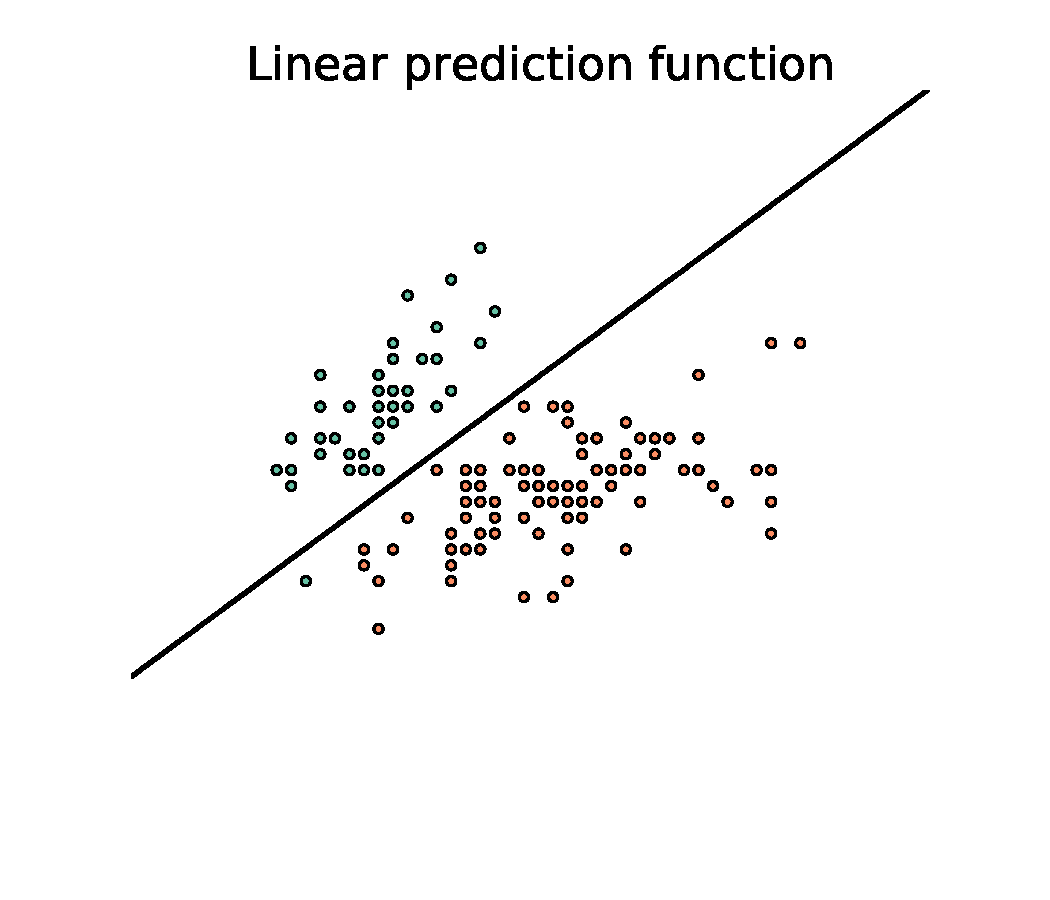
\includegraphics[width=1.3\linewidth]{chapter_2/decision_func_0.pdf}
% \vspace{-20pt}\hspace*{-20pt}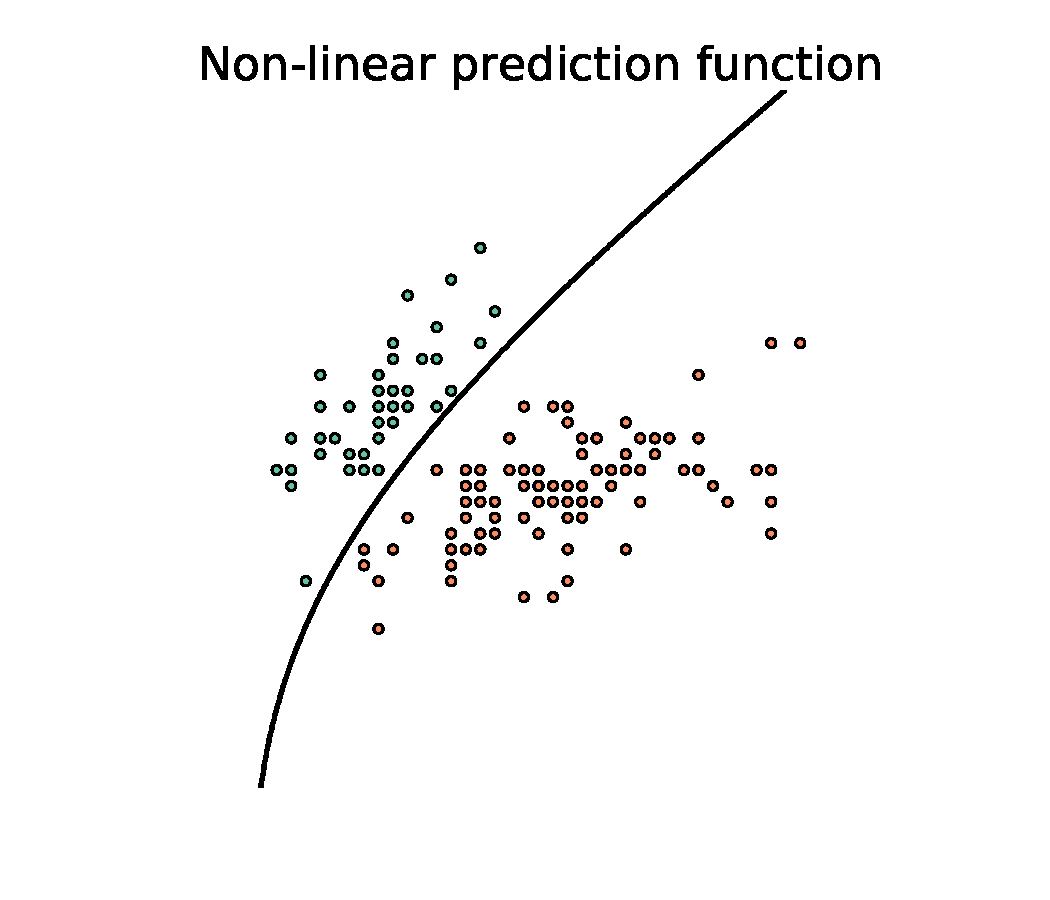
\includegraphics[width=1.3\linewidth]{chapter_2/decision_func_1.pdf}}
% \caption{Example of linear prediction function and non-linear prediction function on a binary classification problem. The classifier will classify all the points on one side of the decision boundary (denoted here with a black line) as belonging to one class and all those on the other side as belonging to the other class. For linear decision functions, the decision surface is an affine function.
% Up: linear SVM showing an affine decision boundary. Down: SVM with polynomial degree 3 kernel, showing a non-linear decision boundary}
% \end{marginfigure}


\begin{marginfigure}
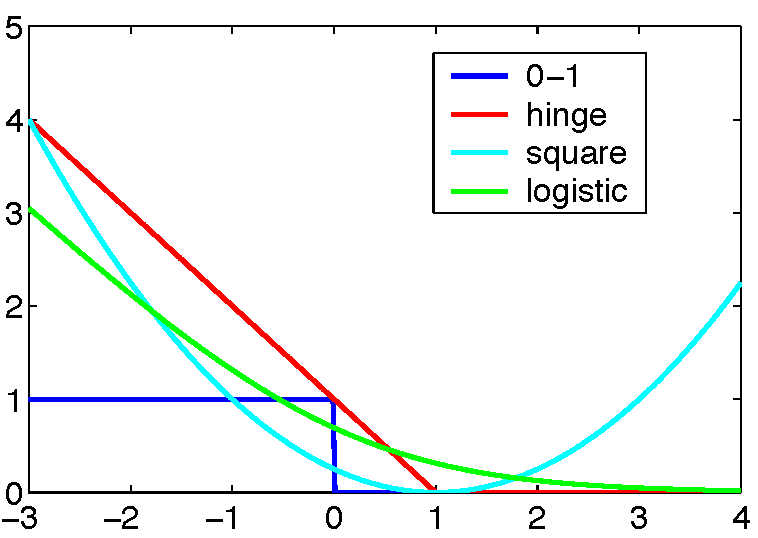
\includegraphics[width=\linewidth]{chapter_2/losses_color.pdf}
\caption{Different surrogate loss functions presented in the text (for y=1): hinge loss, logistic loss and squared loss}
\end{marginfigure}

\newglossaryentry{hinge loss}{name=hinge loss,description=Loss function used by Support Vector Machines}

\begin{itemize}
\item {\it Support Vector Machines (SVM)}. Since its first use in decoding models by~\citet{cox2003}, Support Vector Machines~\citep{Boser:1992:TAO:130385.130401, cortes1995support} have become the reference approach for classification decoding studies. Its success comes from its availability in popular software packages, its overall good performance under a wide array of circumstances~\citep{bottou1994comparison, king1995statlog, caruana2006empirical} and its ability to cope with high-dimensional data. The following surrogate is known as the \emph{\gls{hinge loss}},
\begin{equation} \label{eq:hinge}
\psi(y, \alpha) = \text{max}(1 - y \alpha, 0) \quad .
\end{equation}
Support Vector Machines can be extended to non-linear decision functions through the use of \emph{kernels}~\citep{shawe2004kernel}.


\marginnote{``In the terminology of statistics, this model is known as logistic regression, although it should be emphasized that this is a model for classification rather than regression.'', Christopher M. Bishop (2006). \emph{Pattern Recognition and Machine Learning}.p. 205. }
\item {\it Logistic Regression}. Logistic Regression is a classification model that models the posterior probability as a sigmoid, that is, $P(y|X)$ = $(1 + e^{- y f(X)})^{-1}$. This allows to provide the probability estimates for class membership. The surrogate loss function in this case is given by the negative log-likelihood, that is, also known as the \emph{logistic loss}
\begin{equation}\label{eq:logistic_loss}
\psi(y, \alpha) = \log(1 + \exp({y}\alpha)) ~\quad.
\end{equation}

\item {\it Support Vector Regression}. This is a variant of Support Vector Classification for the regression setting proposed by~\citep{drucker1997support}. The surrogate loss function in this case is known as the \emph{$\varepsilon$-insensitive loss} and is given by
\begin{equation}\label{eq:svr}
\psi(y, \alpha) = \text{max}(|y - \alpha| - \varepsilon, 0) \quad ,
\end{equation}
where $\varepsilon > 0$.


\item {\it Least Squares} is a regression model that minimizes the square of the distance to the prediction. The loss function is given by 
\begin{equation}\label{eq:least_squares}
\psi(y, \alpha) = (y - \alpha)^2 \quad.
\end{equation}
% The values of $\B{w}, c$ that minimize this loss can be computed in closed form as
% $$
% [\hat{\B{w}},~\hat{c}] = \tilde{\B{X}}^{\dagger}\B{y} \quad,
% $$
% where $\tilde{\B{X}}$ is the matrix formed by stacking a column of ones to the original design matrix $\B{X}$.
\end{itemize}


The most popular choice for prediction functions in encoding and decoding models are linear decision functions~\citep{cox2003,laconte2005support, Sutao2011, thirion2006, Naselaris2011}, that is, functions of the form $f(\B{x}) = \text{sgn}(\B{x}^T \B{w} + c)$ for a binary classification problem and $f(\B{x}) = \B{x}^T \B{w} + c$ for a regression problem, where $\B{w} \in \RR^p$ and $c \in \RR$ are unknown parameters to be estimated. 

% These methods assume a linear relationship between the samples and the target variable. We will see in Chapter 5 that pairwise ranking and ordinal regression models can capture a certain degree of non-linearity between the samples and the target variable while maintaining most of the advantages of linear models~\citep{pedregosa:hal-00717990, Doyle2013}.



% It has been found that linear models often outperform non-linear models in the context of decoding \citep{cox2003,laconte2005support, Sutao2011} and encoding studies~\citep{thirion2006, Naselaris2011}.
% However, this supposed superiority can be due to
% an intrinsic linear relationship between the neural
% coding and the cognitive target or simply because the non-linear prediction functions used have not been able to capture the
% true non-linearity of this relationship (e.g. due to lack of training data). 



\subsection{Regularization}\label{subsec:regularization}

Regularization has long played a fundamental role in statistics and related mathematical fields. First introduced by~\citet{tikhonov1977solutions} in the context of solving ill-posed integral equations, it has since become a standard part of the statistical toolkit. 


\begin{marginfigure}
\vspace{10pt}\hspace{-10pt}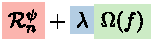
\includegraphics[width=1.\linewidth]{chapter_2/regularization.pdf}
\caption{ The machine learning models that we will consider are estimated as the minimization of a \colorbox{color2}{trade-off} between \colorbox{color1}{data fidelity} and a \colorbox{color3}{regularization} term. Regularization is used to bias the estimated model towards a set of desired solutions.}\label{fig:regularization_formula}
\end{marginfigure}


The purpose of regularization is to use prior knowledge of the problem to bias the estimated model. This can be desirable to solve an ill-posed problem or to avoid overfitting. In this setting, the model is estimated as a solution to an optimization problem of the form
$$
\argmin_{f \in \mathcal{F}} {\mathcal{R}}_n^{\psi}(f) + \lambda \Omega(f) \quad,
$$
where $\Omega(f)$ is the \emph{regularization}, which biases solutions toward a desired kind of solutions and $\mathcal{F}$ is a family of functions (e.g. the family of linear or polynomial functions). In this setting the parameter $\lambda$ controls the trade-off between data-fidelity and the regularization term.

We will present the following penalties due to their widespread use in fMRI analysis. These assume a linear decision function $f$, i.e., $f(\B{x}) = \B{w}^T \B{x} + c$ or $f(\B{x}) = \sign(\B{w}^T \B{x} + c)$ and the penalty will be expressed in terms of the parameters $\B{w}$.


\begin{itemize}

\item {\it squared $\ell_2$} $\left(\Omega(\B{w}) = \|\B{w}\|^2_2 \right)$ . Equivalent to Gaussian normal prior with zero mean~\citep[Chapter 3]{bishop2006pattern}. When loss is linear least squares, it is referred to as Ridge regression and the estimated model $(\hat{\B{w}}, \hat{c})$ has the closed form solution for $\lambda > 0$:
$$
[\hat{\B{w}},~\hat{c}] = (\tilde{\B{X}}^T \tilde{\B{X}} + \lambda n \tilde{\B{I}})^{-1} \tilde{\B{X}}^T \B{y} \quad,
$$
where $\tilde{\B{X}}$ is the matrix formed by stacking a column of ones to the original design matrix $\B{X}$ and $\tilde{\B{I}}$ is the diagonal matrix with all ones except a zero in the last diagonal element, i.e. $\tilde{\B{I}} = \B{I} - \B{e}_n \B{e}_n^T$. This penalty is sometimes also used for computational reasons since it makes the optimization problem better conditioned.

\item {\it $\ell_1$ regularization} $\left(\Omega(\B{w}) = \|\B{w}\|_1 \right)$. Promotes~\emph{sparse} solutions, i.e. solutions with a large fraction of zero coefficients. When combined with a least squares loss function, the model is known as \emph{lasso}~\citep{tibshirani1996regression} and \emph{basis pursuit denoising}~\citep{chen2001atomic}. 

\item {\it elastic-net regularization} $\left(\Omega(\B{w}) = \alpha \|\B{w}\|_1 + (1 - \alpha) \|\B{w}\|^2_2 \right)$. Linearly combines $\ell_1$ and squared $\ell_2$ regularization. In the case of severely correlated variables, the $\ell_1$ penalty tends to select one variable from the group of highly correlated variables and ignore the rest. To mitigate this problem, elastic-net penalty adds a quadratic $\ell_2$ norm to the penalty~\citep{Zou05regularizationand}.

\item {\it total variation (TV)}~\citep{rudin1992nonlinear, chan1999nonlinear, michel2011total}. Total-variation, defined as the $\ell_1$ norm of the gradient promotes piecewise constant solutions. It can be combined with $\ell_1$~\citep{baldassarre2012structured, gramfort:hal-00839984, dohmatob:hal-00991743} and with elastic-net~\citep{dubois2014predictive} penalties. Figure~\ref{fig:tv_reg} compares the estimated coefficients by the use of elastic-net and TV+$\ell_1$ regularization.

% \item {\it nuclear norm regularization} $\left(\Omega(\B{w}) = \|\B{W}\|_* \right)$. This is defined on a matrix.
\end{itemize}

\begin{figure}
\includegraphics[width=1.07\linewidth]{chapter_2/regularization_gramfort.pdf}
\caption{Regularization biases the estimated model towards a desired set of solution. 
In this figure we show the estimated coefficients of a linear model with different regularizations. 
In this model the estimated coefficients correspond to voxels in a brain volume and are displayed over an anatomical image.
In the left, elastic-net regularization yields sparse although very scattered coefficients. Moreover, this regularizer does not take into account the spatial structure of the image. The TV+$\ell_1$ regularization in contrasts yields blobs of nonzero coefficients surrounded zero elements. This latter model has been proved to yield predictive regions which are meaningful from a cognitive point of view. Source: adapted from~\citep{gramfort:hal-00839984}.}\label{fig:tv_reg}
\end{figure}


\vspace{20pt}





\subsection{Model evaluation and cross-validation.}


Since it is possible to construct a classifier that predicts perfectly on the train set but with very poor generalization performance (e.g. the classifier that returns the right label for a sample it has already seen and random otherwise), computing the empirical error on the training set yields a very poor estimator of the true risk of a model.


Cross-validation is a technique to iteratively partition the input dataset in order to obtain a more reliable estimator of the risk~\citep{mosteller1968data, stone1977asymptotics, geisser1975predictive, arlot2010survey}. In this setting a subset of the data is used for training (the \emph{training set}) and the rest of the data is used to compute the accuracy of the trained model (the \emph{test set} or \emph{validation set}). Repeating the process several times and averaging the accuracy of the predictions across the validation sets yields an estimator of the risk. One form of cross-validation leaves out a single observation at a time; this is known as leave-one-out. Another form, known as K-fold cross-validation, splits the data into K subsets; each is held out in turn as the validation set.



The cross-validation score is the average of the empirical risk across all the folds, which is itself an estimator of the risk. This can then be used to perform hypothesis relative to the risk of two predictors $f$ and $g$. For example, consider the test in which we compare the risk of two estimators, that is, $H_0: \mathcal{R}(f) = \mathcal{R}(g)$ and $H_1: \mathcal{R}(f) \neq \mathcal{R}(g)$. This statistical test can be performed using the Wilcoxon signed-rank test presented in Section~\ref{subsec:wilcoxon}. This test takes as input two sequences 
%$\{a_1, \ldots, a_n\}$ and $\{b_1,\ldots, b_n\}$, 
in which the samples are the empirical risk at the different cross-validation folds.

\begin{marginfigure}
\hspace{-10pt}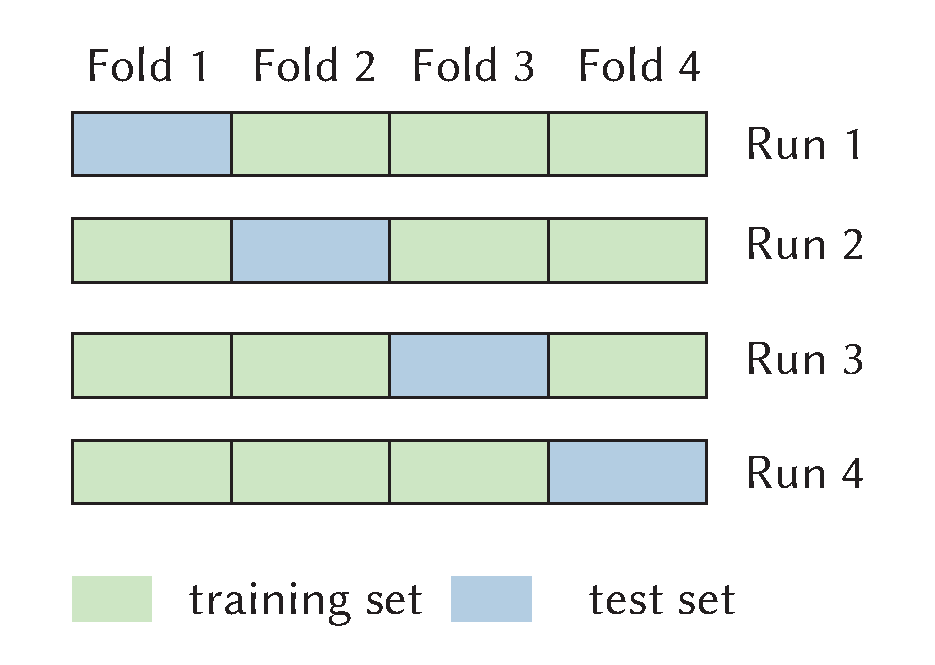
\includegraphics[width=1.2\linewidth]{chapter_2/runs_cv.pdf}
\caption{
	The technique of $K$-Fold cross-validation, illustrated here for the case $K = 4$, involves taking the available data and partitioning it into $K$ groups. Then $K-1$ groups are used (in green) to train a set of models that are then evaluated on the remaining group (in blue). 
}\label{fig:k_fold_cv}
\end{marginfigure}
Cross-validation is an attractive estimator of the risk since it makes no assumptions on the model or the loss function. Alternatives exist for specific loss functions such as Stein's unbiased risk estimate~\citep{stein1981estimation, donoho1995adapting} which is an unbiased estimator of the mean-squared error.

Cross-validation can be used to select the regularization parameter in a setting known as \emph{nested cross-validation}. In this setting, the train set is again split into the different cross-validation folds and the risk associated with the different parameters is computed using this inner cross-validation loop. The procedure can be repeated for the different training sets in the upper-most cross-validation loop. Through this thesis we will use this procedure to estimate the regularization parameter of the different models that we will consider, although it is not the only approach for this purpose. Other methods include Bayesian inference~\citep[Chapter 8 \& 10]{bishop2006pattern} and marginal likelihood maximization~\citep{bock1981marginal}.


% In order to compare different classifiers it is necessary to perform test of the form ``does prediction function $f$ have lower risk than $g$?''. More precisely, the hypothesis are: $H_0: $

% {\blue
% Hypothesis tests concerning the risk of a classifier usually use the cross-validation score as an estimator of the risk. For example, we might want to compare the risk obtained by two different classifiers. It is possible to perform this 
% }

% For example, if the score is a measure whose chance level is at zero, we might want to test the hypothesis that the mean is different from zero. Procedures such as these that test whether the explained variance in a set of data is significantly greater than the unexplained variance are also called \emph{omnibus test}.


% Similarly, it is possible to compare the scores obtained by two different classifiers. For example, we might want to test that the mean scores of the different classifiers are significantly different (equivalently that the difference of scores is different from zero). For these tests, a Wilcoxon signed-rank test can be used~\citep{demvsar2006statistical}.


% \vspace{20pt}{\bf {\sffamily Decoding and encoding problems in the supervised learning framework}}\vspace{10pt}


% In an decoding problem, we seek a model that given an activation coefficients is able to predict the condition associated with that activation coefficient. We can estimate a supervised learning model by considering the training pairs given by the activation coefficients and its respective condition. This way, given a new activation coefficient the learned model will predict a condition, and this can be evaluated using a cross-validation scheme. If the set of stimuli is discrete (e.g. \{houses, faces\} in \citep{haxby2001distributed}) we can use a classification model for this task, if on the other hand the set of stimuli is XXX.



% the sample space is the space of activation coefficients . The activation coefficients for a single condition (as seen in Section~\ref{chapter1_GLM}) have the same dimensions as a brain volume. This volume can be reshaped into a $p$-dimensional vector, with $p$ being the total number of voxels. This transformation eliminates the spatial structure of the activation coefficients, although as we shall see later in this chapter, prior knowledge about the spatial structure of the activation coefficients can be provided in form of~\emph{regularization}. In the 

% {\blue best cross-validation leave-one-session out}





\subsection{fMRI-based brain activity decoding}\label{chap2_decoding}


The paradigm of predicting the stimuli provided to the subject from the concurrent brain activity is known as \emph{brain decoding} and accurate predictions support the hypothesis that the brain activity encodes those stimuli. Early studies \citep{dehaene1998inferring} were able to predict right hand versus left hand movement based on fMRI images. In~\citep{haxby2001distributed, cox2003}, the authors showed that different high-level visual stimulus categories (faces, animals and objects) were associated with distinct patterns of brain activity in visual areas. Subsequent work has shown that decoding can also distinguish many other brain states, for example low-level visual features in the early visual cortex~\citep{haynes2005predicting, kamitani2005decoding} and auditory stimuli in the auditory cortex~\citep{formisano2008saying, staeren2009sound}, as well as more abstract brain states such as intentions~\citep{haynes2007reading, soon2008unconscious} and the contents of working memory~\citep{harrison2009decoding}. 



\begin{figure}
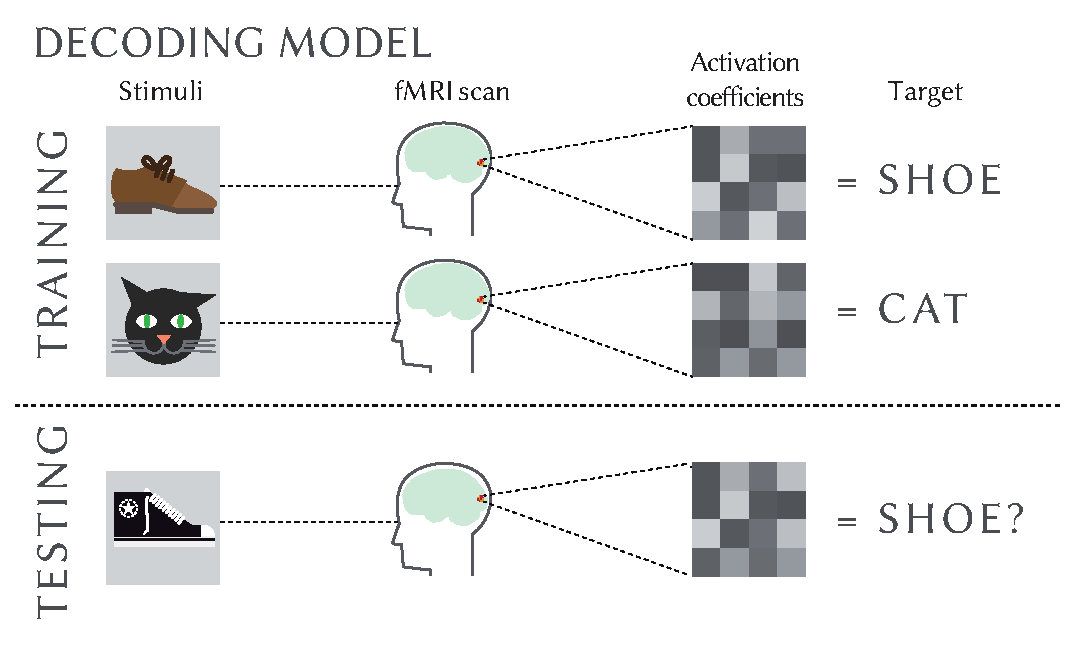
\includegraphics[width=1.05\linewidth]{chapter_2/decoding2.pdf}
\caption{Decoding models use patterns of activity to discriminate between cognitive states. Different \gls{activation coefficient}s reflect different mental states; for example, those associated with different images viewed by the subject. In a training phase, the classifier will learn to discriminate between activity patterns measured under different cognitive states. In the testing phase the generalization performance of the trained model is quantified by evaluating the classifier on the testing set and comparing the output of the classifier with the true labels associated with the stimuli. Adapted from~\citep{smith2013reading}.}\label{fig:c2_decoding}
\end{figure}

% This decoding approach can be used to provide answers to some neuroscientific questions. This question is a hypothesis testing problem that can be studied both on a single subject or a multi-subject study. In the first case the inference that we want to establish is whether the classifier designed on data from a given brain area of one subject is accurate enough to claim that the area actually encodes some information about the stimuli. 

The neuroscientific questions that brain decoding is able to address are commonly shaped within the statistical hypothesis testing framework. The inference that we want to establish is whether the classifier designed on data from a given brain area of one subject is accurate enough to claim that the area encodes some information about the stimuli. In this setting, the null hypothesis is that a given brain area does not contain stimuli-related information. The ability of the classifier to correctly predict some information about the stimulus is considered a positive evidence in support of the alternate hypothesis of presence of stimuli-related information within the brain activity.



% Although it is possible to perform decoding directly on raw BOLD
% signal~\citep{Mourao-Miranda2007, miyawaki2008visual}, the common approach consists in extracting the activation coefficients from
% the BOLD signal by using a known form of the Hemodynamic Response Function and the linear-time-invariant property of BOLD signal\label{chapter1_GLM} described in section \ref{chapter1_GLM} and use this estimates as input to the decoding model. 


% Compared to Statistical Parametric Maps, decoding models offer the advantage that the model relating activation coefficients to stimuli can consider several voxels at the same time ({\blue not making the same inference!!}). In the literature the decoding model is often described as a multi-variate approach while SPMs are univariate approaches. Multi-variate approaches have the advantage that they are able to discriminate conditions based on a distributed pattern of activity, contrary to univariate approaches that can only discriminate conditions based on a single activation coefficient. {\blue This translates in greater statistical power but also in a higher risk of overfitting due to the high dimensionality of the activation coefficients. In these settings the the number of voxels (dimensions) is typically higher than the number of activation coefficients (samples), thus the use of regularization and/or dimensionality reduction approaches is necessary}.



In~\citep{borghesani:hal-00986606}, we have used decoding models to establish in which regions of the brain it is possible to decode different aspects of words representing real-world objects. One of the tasks was to decode the size of items from the words representing those objects. In this case, the different stimuli are ordered according to their relative size, so the target variable is of ordinal nature. We predict the target variable from the brain activation on 6 anatomically defined regions of interest (ROI, which correspond to different Brodman areas). The metric is Kendall tau, which is a measure of the association between two measured quantities. This metric lies between -1 and 1. This metric and the used model will be presented in full detail in Chapter~\ref{chap:decoding_ordinal}).

% The Ridge regularization parameter chosen by nested cross-validation and the scores reported are the cross-validations scores using a leave-one-session out scheme.

\begin{figure*}
\mbox{
{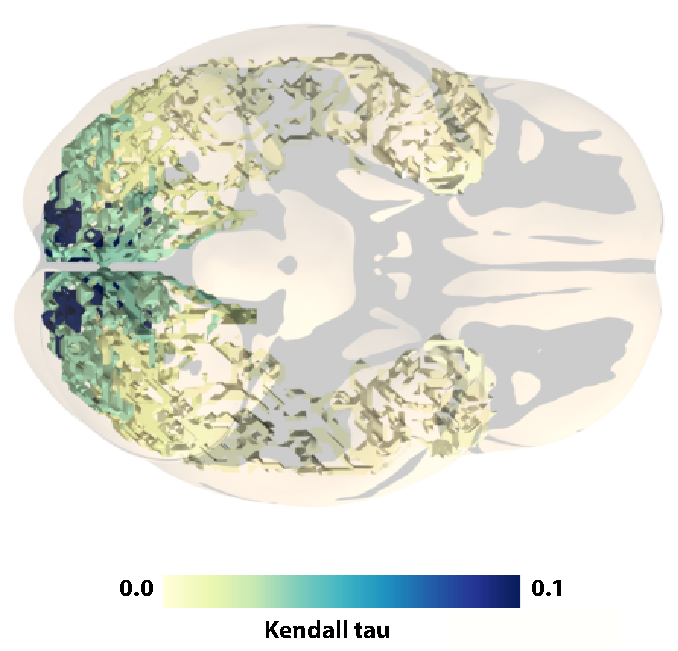
\includegraphics[width=0.40\linewidth]{chapter_2/word_length_horiz.pdf}}
{\hspace{1cm}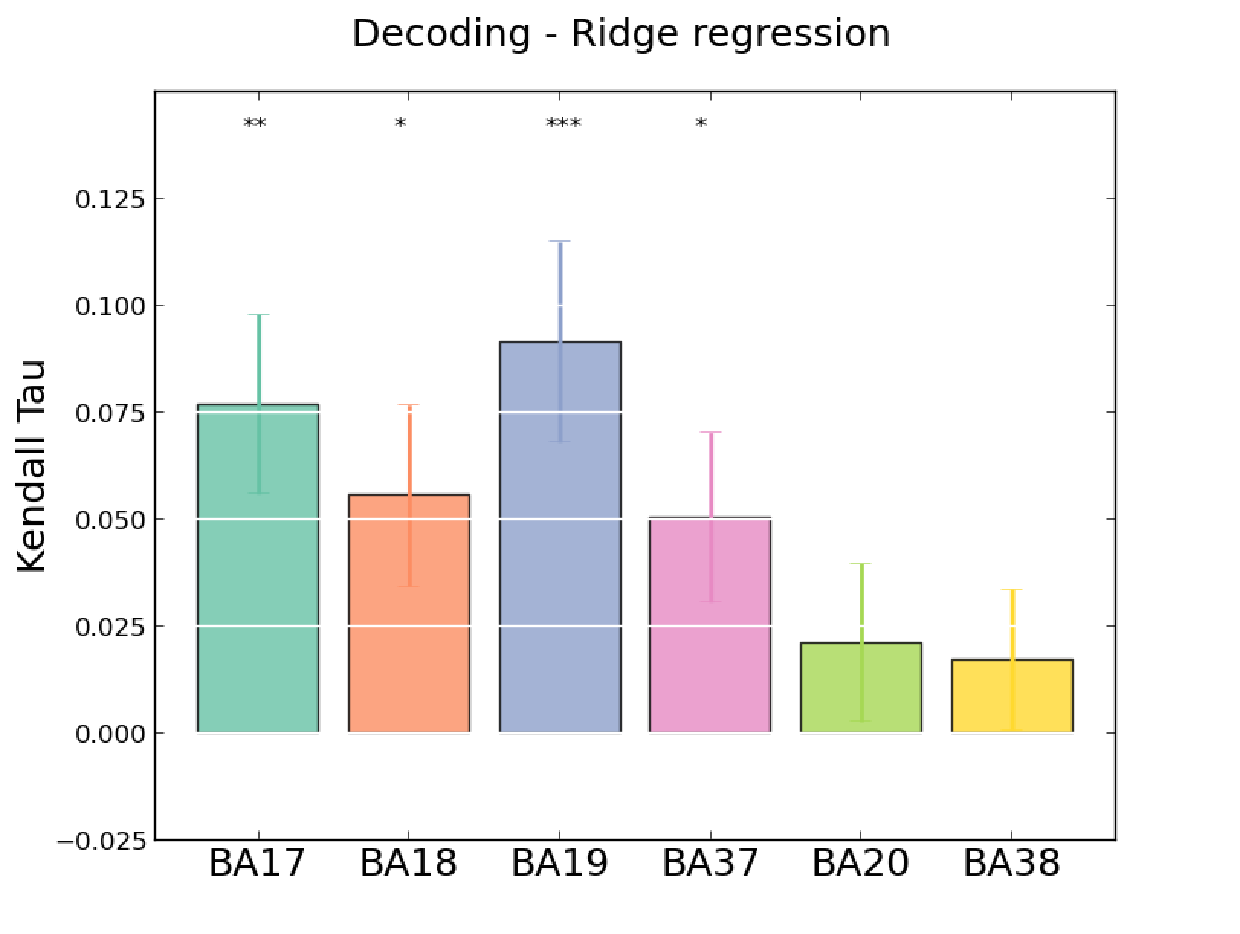
\includegraphics[width=0.55\linewidth]{chapter_2/vb_decode_size.png}}
}
\caption{Cross-validation scores for the prediction of the length of words from~\citep{borghesani:hal-00986606}. The metric is Kendall tau (higher is better). In the left, the same scores are depicted for the different regions (Brodman areas). 
}\label{fig:brain_score_length_vb}
\end{figure*}


As can be seen in Figure~\ref{fig:brain_score_length_vb}, this decoding model results in a higher decoding score in primary and secondary visual areas. In this case, a Wilcoxon signed-rank test was used to asses the statistical significance ($p$-value $< 0.05$) of the scores. This is denoted by the $*$ symbol that reflects the significance of a Wilcoxon test that the mean is significantly different than zero, $*$ = $p$-val $< 0.05$, $**$ = $p$-val $< 10^{-3}$, $***$ = $p$-val $< 10^{-6}$. This is achieved in Brodman areas BA17, BA18 and BA19. This experiments allows us to establish that the aforementioned areas encode some information related to the size of the stimuli.




% it is possible to decode the size of  objects from its conceptual representation (recall that stimuli are words and not images) in the aforementioned brain regions.

% {\blue Decoding vs statistical inference}. Although related, decoding and the application of classical inference to fMRI detailed before answer slightly different questions.  From a cognitive point of view, one of the main advantages of decoding models over classical inference {\blue is that they are able to use information from multiple voxels at the same time}.



\subsection{fMRI-based brain activity encoding}\label{chap2_encoding}

fMRI-based \emph{encoding} models (also known as \emph{voxel-wise modelling}) \citep{thirion2006, Kay2008, mitchell2008predicting}, seek to predict the patterns of brain activity from the the stimuli features. A machine learning model is learned from the stimuli features to the \gls{activation coefficient}s of a single voxel.
%\marginnote{Although it would be possible to construct encoding models that predict a set of voxels simultaneously, the models that have appeared in the literature until now consider the different voxels separately.} 
The sample space in this case is the space of features derived from the stimuli, e.g. spatial Dirac functions in~\citep{thirion2006} or Gabor filters in the case of natural images~\citep{Kay2008, Naselaris2014}. The predicted activation coefficient can then be compared to the true activation coefficient measured on left out data by using some distance metric such as Pearson or Spearman correlation coefficient.

% {\blue What inference can you make with encoding models ?}

\begin{figure}
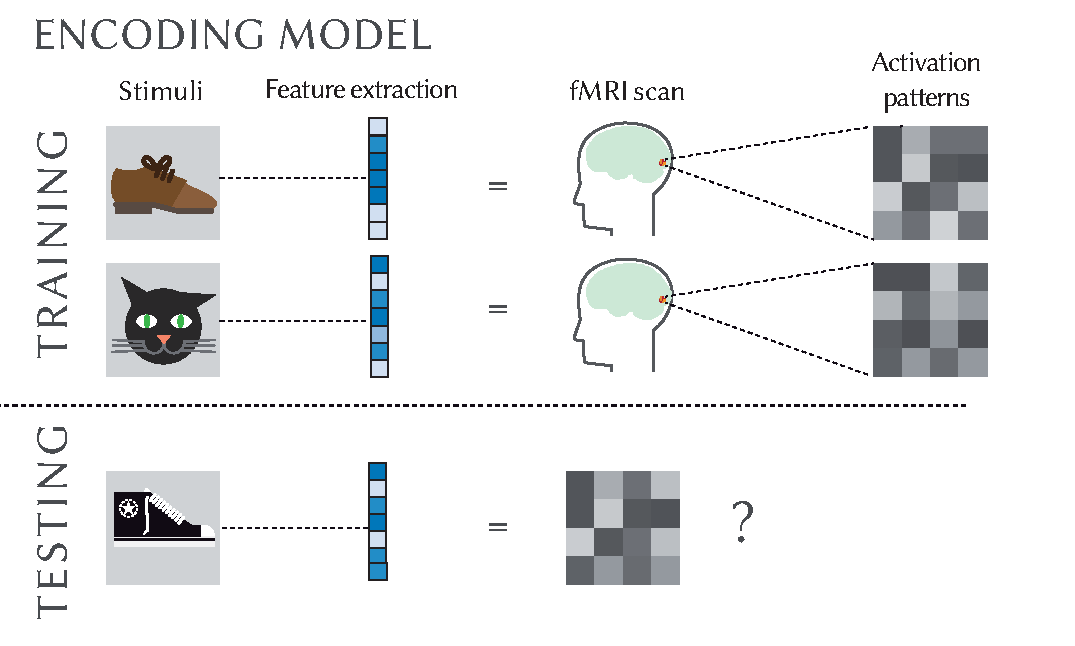
\includegraphics[width=1.\linewidth]{chapter_2/encoding.pdf}
\caption{ In an encoding model the patterns of brain activity are predicted by a machine learning model based on the stimuli features. The sample space in this case is the space of features derived from the stimuli, e.g. a set of Gabor filters in~\citep{Kay2008}. The predicted activation coefficient can then be compared to the true activation coefficient measured on left out data by using some distance metric such as Pearson's correlation coefficient. Adapted from~\citep{smith2013reading}.}\label{fig:c2_encoding}
\end{figure}

To the best of my knowledge, all of the encoding models that have been
published in the literature make assume a use of linear relationship features to the activation coefficients. That is, they assume that there is a  mapping from the stimulus space to the feature space that, and a linear mapping between the feature space and the activity space. However, the success of an encoding model depends in great measure on deriving the right features from the stimuli, a transformation that might be nonlinear. For example, \citet{naselaris2009bayesian} constructed two different models for each voxel: a model based on phase-invariant Gabor wavelets, and a semantic model that was based on a scene category label for each natural scene. The authors showed that the Gabor wavelet model provided good predictions of activity in early visual areas, while the semantic model predicted activity at higher stages of visual processing. 

Encoding and decoding can be seen as complementary operations: while encoding uses stimuli to predict activity,  decoding uses activity to predict information about the stimuli. Furthermore, encoding offers the advantage over decoding models that they can be used to predict information about an unseen stimuli. In this setting encoding models have been used to reconstruct stimuli from brain activity patterns in~\citep{miyawaki2008visual, naselaris2009bayesian, nishimoto2011reconstructing}. A similar setting was used in~\citep{Kay2008} to identify natural images. Here, the predicted activation coefficients were used to select the image that matched most closely the measured activation coefficients.



\section{Conclusion}

In this chapter we  have presented the statistical methods that will be used for drawing conclusions from fMRI experiments in further chapters. The chapter is divided into two sections. In the first section we have introduced the framework of statistical hypothesis testing and presented several parametric and non-parametric tests. We have presented an application of voxel-wise hypothesis testing known as Statistical Parametric Maps (SPMs).



In the second part of this chapter we have presented the setting of supervised learning. We described different surrogate loss functions and penalties that have found applications in the context of fMRI analysis. The surrogate loss functions that we described are  as Support Vector Machines, Logistic Regression, Support Vector Regression and Least Squares. The penalties that we have present are: squared $\ell_2$, $\ell_1$, elastic-net ($\ell_2^2 + \ell_1$) and total-variation (TV). Finally, we present two neuroscientific problems that can be model as a supervised learning problem: \emph{encoding} and \emph{decoding}.


\newpage


\begin{fullwidth}
\bibliographystyle{plainnat}
\bibliography{chapter_2/biblio2}
\end{fullwidth}
